% !TeX program = xelatex
\documentclass[12pt,a4paper]{exam-zh}

\usepackage{amsmath,array,graphicx,booktabs,multirow}
\usepackage{enumitem}
\usepackage{fancyhdr}
\usepackage{tikz}
\usepackage{tabularx}
\usepackage{setspace}
\setCJKmainfont{Noto Serif CJK SC}
\geometry{margin=2.2cm,top=2.0cm,bottom=2.2cm}
\pagestyle{fancy}
\fancyhf{}
\cfoot{-\thepage{}-}
\renewcommand{\headrulewidth}{0pt}
\renewcommand{\footrulewidth}{0pt}
\setlength{\parindent}{0pt}
\setlength{\parskip}{0.2em}
\setlength{\headheight}{14pt}
\linespread{1.12}
\usepackage{setspace}
\usepackage{eso-pic}
\usetikzlibrary{calc,angles,quotes}

%region exam setup

\examsetup{
    page = {
    size = a4paper,           % 设定纸张大小 [4]
    foot-content = { - ; - }  % 页脚显示为 -1-, -2- 格式 [3]
  },
    choices = {
    label-pos = top-left,
    column-sep = 1em,
    label-pos = auto,
    label-sep = 0.5em,
    max-columns = 4
    },
  question = {
    top-sep    = 1em, % 调整题目上方的垂直距离（默认值为 .5em plus .5em minus .2em）
    bottom-sep = 1em  % 调整题目下方的垂直距离（默认值为 .5em plus .5em minus .2em）
  },
    paren = {
    show-paren = false  % 设置为 false 则不显示括号 [3, 4]
  },
    choices = {
    label = \textbf{\Alph*}
  }, 
    solution = {
    show-solution = show-move, % 答案自动移动到卷末
    label-content = {参考答案},  % 答案区的标题文字
    show-qed = true            % 在解答末尾显示结束符号 ◻ 
  }
}

\newcommand{\qscoreoffset}{4em}
\newlist{questionparts}{enumerate}{1}
\setlist[questionparts]{
    label=(\alph*),
    itemsep=0.5em,
    leftmargin=2em,
    rightmargin=4em,
    before={\renewcommand{\qscoreoffset}{8em}},
}
\newcommand{\qscore}[2][\%]{%
    \leavevmode\unskip\nobreak\hfill
    \makebox[0pt][l]{\makebox[\qscoreoffset][r]{(#2#1)}}%
}

% 仅用于参考答案：保持字号，缩小行距与公式间距。
\newcommand{\compactanswers}{%
    \setstretch{1.0}%
    \setlength{\parskip}{2pt}%
    \setlength{\abovedisplayskip}{4pt}%
    \setlength{\belowdisplayskip}{4pt}%
    \setlength{\abovedisplayshortskip}{2pt}%
    \setlength{\belowdisplayshortskip}{3pt}%
    \setlength{\jot}{2pt}%
    \setlist[enumerate]{itemsep=3pt,parsep=0pt,topsep=3pt,partopsep=0pt}%
}
%endregion


%region 卷面变量设置
    % ==========================
    % 兼容从当前文件夹或工作区根目录进行编译
    % ==========================
% 卷面变量设置（只需改这里）
% ==========================
\newcommand{\papercode}{SC 07}
\newcommand{\examtitle}{2026年金宝培元独立中学毕业考}
\newcommand{\examlevel}{高中组}
\newcommand{\examsubject}{高级数学(I)}
\newcommand{\sidebartext}{高级数学(I)/一}
\newcommand{\papername}{试卷二}
\newcommand{\papertype}{作答题}
\newcommand{\examdate}{2026年9月24日}
\newcommand{\examtime}{9.15 a.m.－11.15 a.m.}
\newcommand{\examduration}{2小时}
\newcommand{\questionpages}{4面}
\newcommand{\paperonepercentage}{30\%}
\newcommand{\papertwopercentage}{70\%}
\newcommand{\setterteacher}{蔡杰庆师}
\newcommand{\reviewteacher}{杨丽芳师}
\newcommand{\auditteacher}{雷泳健师}


    \newcommand{\optrow}[4]{%
    \begin{tabular*}{\linewidth}{@{\extracolsep{\fill}}llll}
    A~#1 & B~#2 & C~#3 & D~#4
    \end{tabular*}%
    }
    \newcommand{\qitem}[5]{\item #1\par\optrow{#2}{#3}{#4}{#5}}
%endregion
    \begin{document}


%region 封面
    \AddToShipoutPictureFG*{%
    \begin{tikzpicture}[remember picture,overlay]
        \node[
            anchor=north west,
            fill=black,
            minimum width=22pt,
            minimum height=90pt,
            inner sep=0pt
        ] (sidebar) at ([xshift=3em,yshift=-3em]current page.north west) {};
        \node[
            rotate=270,
            text=white,
            font=\bfseries\footnotesize
        ] at (sidebar.center) {\sidebartext};
    \end{tikzpicture}%
    \put(24,18){\makebox(0,0)[lb]{\small 版权所有}}%
    \put(520,18){\makebox(0,0)[lb]{\bfseries\small 【机密】}}%
    }

    \thispagestyle{fancy}

    \begin{minipage}[t]{0.22\linewidth}
    \vspace{0pt}
    \end{minipage}
    \hfill
    \begin{minipage}[t]{0.8\linewidth}
        \centering
        {\zihao{2}\bfseries \examtitle\par}
        \vspace{0.5em}
        {\zihao{3}\bfseries \examlevel\par}
        \vspace{0.5em}
        {\zihao{2}\bfseries \examsubject\par}
        \vspace{0.1em}
        {\large (\papercode)\par}
    \end{minipage}
    \hfill
    \begin{minipage}[t]{0.18\linewidth}
    \vspace{0pt}
    \end{minipage}



    \begin{center}
    \begin{tabular}{l}
        \multicolumn{1}{c}{\papername\hspace{2em}\papertype}\\[-0.1em]
        \midrule
        日期：\examdate\\[-0.1em]
        时间：\examtime\\[-0.1em]
        \multicolumn{1}{c}{(\examduration)}\\
        \midrule
    \end{tabular}
    \end{center}


    {\zihao{4}\bfseries \underline{考生须知}\par}
    \vspace{0.3em}

    {\setstretch{1.0}
    \begin{enumerate}[label=（\chinese*）,leftmargin=3em,itemsep=0.25em,topsep=0.3em,parsep=0pt,partopsep=0pt]
    \item 本科试卷共分两份：\\
    \hspace*{2em}试卷一：选择题（\paperonepercentage）；\\
    \hspace*{2em}试卷二：作答题（\papertwopercentage）。

    \item 试卷二：作答题 \\
        \hspace*{2em}第 1 题至第 5 题（4\%）；\\
        \hspace*{2em}第 6 题至第 10 题（6\%）；\\
        \hspace*{2em}第 11 题至第 12 题（10\%）。\\
        \hspace*{2em}12 题全答

  \item \textbf{每题必须用新的一张纸作答。}

  \item 只可用蓝色或黑色的原子笔书写，惟可用铅笔画图。

  \item 不必抄题，惟试题号码必须书写清楚。

  \item 所有演算必须清楚地写出。必要的几何图形必须画出。

  \item 可使用所规定的电子计算机进行演算，除非题目限制。

  \item 答卷必须依试题号码次序排列，并且将\textbf{积分表}（电脑卡）置于上\\
  面，合订成一本。

  \item 试卷二作答题共印\questionpages，最后一面空白。
    \end{enumerate}
    }

    \vspace{0.5em}

    \begin{center}
    {% 外框粗细及外、内框之间的距离
    \setlength{\fboxrule}{3pt}%
    \setlength{\fboxsep}{1.5pt}%
    \fbox{%
        {% 内框粗细及文字与内框之间的距离
        \setlength{\fboxrule}{0.5pt}%
        \setlength{\fboxsep}{6pt}%
        \fbox{\rule{0pt}{1.1em}\hspace{1.2em}{\zihao{4}\bfseries 未经正式宣布\quad 不得翻看内页}\hspace{1.2em}}%
        }%
    }%
    }
    \end{center}

    \vfill

    \begin{tabular*}{\linewidth}{@{\extracolsep{\fill}}ll}
    考生姓名：\underline{\hspace{4.2cm}} & 考生编号：\underline{\hspace{4.0cm}}
    \end{tabular*}

%endregion

\newpage
%region 范围：2026年金宝培元独中高三高级数学(SC05)毕业考·试卷二·甲组 | 考点：无理方程的解法 | 难度：中等
\begin{question}[points = 4]
    解方程 $\sqrt{x^2+11}-\sqrt{x^2+4}=1$。
    \qscore{4}
\end{question}

\begin{solution}
    \begingroup\compactanswers
    解方程 $\sqrt{x^2+11}-\sqrt{x^2+4}=1$。 \\
    设 $a=\sqrt{x^2+11}$，$b=\sqrt{x^2+4}$，利用平方差公式建立方程组。 \\
    \[
        a-b=1
    \tag*{(1分)}
    \]
    \begin{align*}
        a^2-b^2 &= (x^2+11)-(x^2+4) \\
        &= 7 \\
        (a-b)(a+b) &= 7 \\
        a+b &= 7
    \tag*{(1分)}
        \end{align*}
    \begin{align*}
        2a &= 8 \\
        a &= 4,\quad b=3
    \tag*{(1分)}
        \end{align*}
    \begin{align*}
        a^2 &= x^2+11 \\
        16 &= x^2+11 \\
        x^2 &= 5
    \end{align*}
    检验：$b^2=x^2+4=9$，与 $b=3$ 相符。
    \[
        x = \pm\sqrt{5}
    \tag*{(1分)}
    \]
    \par\endgroup
\end{solution}
%endregion

% %region 范围：2026年金宝培元独中高三高级数学(SC05)毕业考·试卷二·甲组 | 考点：立体几何——直线与平面所成的角 | 难度：中等
% \begin{question}[points = 4]
%     图1中的立体 $ABCD$-$EFGH$ 是一个长方体，其中 $AB:BC:CG=6:4:1$。点 $P$ 在 $AB$ 上，且 $AP:PB=2:1$。

%     \begin{center}
%         \begin{tikzpicture}[scale=0.75]
%             \coordinate (A) at (0,0);
%             \coordinate (B) at (6,0);
%             \coordinate (C) at (8.4,1.6);
%             \coordinate (D) at (2.4,1.6);
%             \coordinate (E) at (0,2.2);
%             \coordinate (F) at (6,2.2);
%             \coordinate (G) at (8.4,3.8);
%             \coordinate (H) at (2.4,3.8);
%             \coordinate (P) at (4,0);

%             \draw[dashed] (A)--(D);
%             \draw[dashed] (D)--(C);
%             \draw[dashed] (D)--(H);
%             \draw[dashed] (H)--(E);
%             \draw[dashed] (H)--(G);

%             \draw (A)--(B)--(C)--(G)--(F)--(E)--cycle;
%             \draw (B)--(F);
%             \draw (C)--(G);

%             \fill (A) circle (1.5pt) node[below left]{$A$};
%             \fill (B) circle (1.5pt) node[below right]{$B$};
%             \fill (C) circle (1.5pt) node[right]{$C$};
%             \fill (D) circle (1.5pt) node[above left]{$D$};
%             \fill (E) circle (1.5pt) node[left]{$E$};
%             \fill (F) circle (1.5pt) node[right]{$F$};
%             \fill (G) circle (1.5pt) node[above right]{$G$};
%             \fill (H) circle (1.5pt) node[above left]{$H$};
%             \fill (P) circle (1.5pt) node[below]{$P$};
%         \end{tikzpicture}
%     \end{center}

%     \begin{questionparts}
%         \item 求平面 $HGP$ 与平面 $ABCD$ 的夹角。（答案准确至 $0.01^\circ$） \qscore{2}

%         \item 不通过计算，解释如何能判断 $\angle GPC$ 与 $\angle HPD$ 何者较大。 \qscore{2}
%     \end{questionparts}
% \end{question}

% \begin{solution}
%     \begin{enumerate}[label=(\alph*)]
%         \item 求平面 $HGP$ 与平面 $ABCD$ 的夹角。 \\
%         以 $A$ 为原点建立空间直角坐标系，求两平面法向量的夹角。 \\
%         设 $A(0,0,0)$，$B(6,0,0)$，$C(6,4,0)$，$D(0,4,0)$，$E(0,0,1)$，$F(6,0,1)$，$G(6,4,1)$，$H(0,4,1)$，$P(4,0,0)$。
%         \begin{align*}
%             \overrightarrow{GH} &= (-6,0,0) \\
%             \overrightarrow{GP} &= (-2,-4,-1) \\
%             \mathbf{n_1} &= \overrightarrow{GH}\times\overrightarrow{GP} = (0,-6,24)
%         \end{align*}
%         \qscore[分]{1} \\
%         平面 $ABCD$ 的法向量 $\mathbf{n_2}=(0,0,1)$。
%         \begin{align*}
%             \cos\theta &= \frac{|\mathbf{n_1}\cdot\mathbf{n_2}|}{|\mathbf{n_1}||\mathbf{n_2}|} \\
%             &= \frac{24}{\sqrt{612}} = \frac{4\sqrt{17}}{17} \\
%             \theta &\approx 14.04^\circ
%         \end{align*}
%         \qscore[分]{1}

%         \item 判断 $\angle GPC$ 与 $\angle HPD$ 何者较大。 \\
%         利用 $PC$、$PD$ 的相对大小及公共高 $CG=DH$ 判断正切值大小。
%         \begin{align*}
%             PC^2 &= PB^2+BC^2 = 2^2+4^2=20 \\
%             PD^2 &= PA^2+AD^2 = 4^2+4^2=32
%         \end{align*}
%         故 $PC<PD$。
%         \qscore[分]{1} \\
%         由于 $CG=DH$（长方体侧棱等长），
%         \[
%             \tan\angle GPC=\frac{CG}{PC},\quad \tan\angle HPD=\frac{DH}{PD}
%         \]
%         $PC<PD \Rightarrow \tan\angle GPC>\tan\angle HPD$，故 $\angle GPC>\angle HPD$。
%         \qscore[分]{1}
%     \end{enumerate}
% \end{solution}
% %endregion

%region 范围：2026年金宝培元独中高三高级数学(SC05)毕业考·试卷二·甲组 | 考点：直线方程与垂足坐标 | 难度：中等
\begin{question}[points = 4]
    已知三点 $A(4,6)$，$B(-3,5)$ 及 $C(9,-4)$。点 $P$ 是由点 $A$ 到 $BC$ 边上的高的垂足。求点 $P$ 的坐标。
    \qscore{4}
\end{question}

\begin{solution}
    \begingroup\compactanswers
    求点 $A$ 到直线 $BC$ 的垂足 $P$ 的坐标。 \\
    设 $P$ 为直线 $BC$ 上一点，利用 $\overrightarrow{AP}\perp\overrightarrow{BC}$ 求参数。 \\
    设 $\overrightarrow{BC}=(12,-9)$，$P=B+t\overrightarrow{BC}=(-3+12t,\ 5-9t)$。
    \qscore[分]{1}\par
    \begin{align*}
        \overrightarrow{AP} &= (-7+12t,\ -1-9t)
    \end{align*}
    由 $\overrightarrow{AP}\cdot\overrightarrow{BC}=0$：
    \begin{align*}
        12(-7+12t)-9(-1-9t) &= 0 \\
        -84+144t+9+81t &= 0 \\
        225t &= 75
    \tag*{(1分)}
        \end{align*}
    \begin{align*}
        t &= \frac{1}{3}
    \tag*{(1分)}
        \end{align*}
    \begin{align*}
        P &= \left(-3+12\times\frac13,\ 5-9\times\frac13\right) \\
        &= (1,\ 2)
    \tag*{(1分)}
        \end{align*}
    \par\endgroup
\end{solution}
%endregion

%region 范围：2026年金宝培元独中高三高级数学(SC05)毕业考·试卷二·甲组 | 考点：古典概率与组合计数 | 难度：中等
\begin{question}[points = 4]
    一盒子内有 4 粒红球，5 粒黄球及 8 粒蓝球。若从盒子中随机拿出两粒球，求这两粒球颜色不同的概率。
    \qscore{4}
\end{question}

\begin{solution}
    \begingroup\compactanswers
    求随机取出两粒球颜色不同的概率。 \\
    盒中共 17 粒球，用组合数计算总取法与同色取法。
    \[
        \text{总取法} = \binom{17}{2}=136
    \tag*{(1分)}
    \]
    \begin{align*}
        \text{同色取法} &= \binom{4}{2}+\binom{5}{2}+\binom{8}{2} \\
        &= 6+10+28 \\
        &= 44
    \tag*{(1分)}
        \end{align*}
    \begin{align*}
        \text{不同色取法} &= 136-44 \\
        &= 92
    \tag*{(1分)}
        \end{align*}
    \begin{align*}
        P(\text{不同色}) &= \frac{92}{136} \\
        &= \frac{23}{34}
    \tag*{(1分)}
        \end{align*}
    \par\endgroup
\end{solution}
%endregion

%region 范围：2026年金宝培元独中高三高级数学(SC05)毕业考·试卷二·甲组 | 考点：复合函数（对数函数）求导 | 难度：中等
\begin{question}[points = 4]
    已知 $y=\ln(4x^2+3x)$，求 $\dfrac{dy}{dx}$。
    \qscore{4}
\end{question}

\begin{solution}
    \begingroup\compactanswers
    求 $y=\ln(4x^2+3x)$ 的导数。 \\
    利用复合函数求导法则 $\dfrac{d}{dx}\ln u=\dfrac{u'}{u}$。 \\
    设 $u=4x^2+3x$。
    \begin{align*}
        u' &= 8x+3
    \tag*{(1分)}
        \end{align*}
    \begin{align*}
        \frac{dy}{dx} &= \frac{u'}{u}
    \tag*{(1分)}
        \end{align*}
    \begin{align*}
        \frac{dy}{dx} &= \frac{8x+3}{4x^2+3x}
    \tag*{(2分)}
        \end{align*}
    \par\endgroup
\end{solution}
%endregion

%region 范围：2026年金宝培元独中高三高级数学(SC05)毕业考·试卷二·乙组 | 考点：反函数 | 难度：中等偏难
\begin{question}[points = 4]
    已知函数 $f(x)=a+\dfrac{b}{x+5}$ 且 $f(-4)=-1$，$f(-1)=2$。求 $f^{-1}(x)$。 \qscore{4}
\end{question}

\begin{solution}
    \begingroup\compactanswers
        求 $f^{-1}(x)$。 \\
        代入已知条件建立方程组求 $a,b$。
        \begin{align*}
            f(-4)=a+\frac{b}{1}&=-1 \\
            f(-1)=a+\frac{b}{4}&=2
        \tag*{(1分)}
        \end{align*}
        解方程组：
        \begin{align*}
            a+b&=-1 \\
            a+\frac{b}{4}&=2
        \end{align*}
        两式相减：$-\dfrac{3b}{4}=-3 \Rightarrow b=4$，代入得 $a=-5$... \\
        （重新代入验证）$a=-1-b=-1-4=-5$？验证 $f(-1)=-5+1=-4\ne2$，故重新求解：
        \begin{align*}
            \left(a+\frac{b}{4}\right)-(a+b) &= 2-(-1) \\
            -\frac{3b}{4} &= 3 \\
            b &= -4
        \end{align*}
        代回 $a+b=-1$：$a=-1-(-4)=3$。
        \qscore[分]{1}\par
        故 $f(x)=3-\dfrac{4}{x+5}$。设 $y=3-\dfrac{4}{x+5}$，解出 $x$：
        \begin{align*}
            y-3&=-\frac{4}{x+5} \\
            x+5&=\frac{-4}{y-3} \\
            x&=\frac{-4}{y-3}-5
        \tag*{(1分)}
        \end{align*}
        化简：
        \[
            f^{-1}(x)=\frac{-4-5(x-3)}{x-3}=\frac{11-5x}{x-3},\quad x\ne3
        \tag*{(1分)}
    \]
    \par\endgroup
\end{solution}
%endregion

%region 范围：2026年金宝培元独中高三高级数学(SC05)毕业考·试卷二·乙组 | 考点：含平方因式的分式不等式、二项式定理 | 难度：中等偏难
\begin{question}[points = 6]
    \begin{questionparts}
        \item 解不等式 $\dfrac{(x+1)^2(2-x)}{x-3}\le 0$。 \qscore{3}

        \item 求 $\left(x^3-\dfrac{1}{2x}\right)^{10}$ 展开式中 $x^2$ 的系数。 \qscore{3}
    \end{questionparts}
\end{question}

\begin{solution}
    \begingroup\compactanswers
    \begin{enumerate}[label=(\alph*)]
        \item 解不等式 $\dfrac{(x+1)^2(2-x)}{x-3}\le 0$。 \\
        由于 $(x+1)^2\ge0$ 恒成立（$x=-1$ 时等号成立），故只需讨论 $\dfrac{2-x}{x-3}\le0$ 的符号（$x=-1$ 时整式为 $0$，已满足）。
        \qscore[分]{1}\par
        令临界点 $x=2,\ x=3$，分区间检验 $\dfrac{2-x}{x-3}$ 的正负：
        \[
            x<2:\ (+)/(-)<0;\quad 2<x<3:\ (-)/(-)>0;\quad x>3:\ (-)/(+)<0
        \tag*{(1分)}
    \]
        综合（含 $x=-1$ 已在 $x\le2$ 范围内，$x=3$ 使分母为零须排除）：
        \[
            x\in(-\infty,\,2]\cup(3,\,\infty)
        \tag*{(1分)}
    \]

        \item 求 $\left(x^3-\dfrac{1}{2x}\right)^{10}$ 展开式中 $x^2$ 的系数。 \\
        通项：
        \[
            T_{r+1}=\binom{10}{r}(x^3)^{10-r}\left(-\frac{1}{2x}\right)^r=\binom{10}{r}\left(-\frac12\right)^r x^{30-4r}
        \tag*{(1分)}
    \]
        令 $30-4r=2$：
        \[
            r=7
        \tag*{(1分)}
    \]
        系数：
        \[
            \binom{10}{7}\left(-\frac12\right)^7=120\times\left(-\frac{1}{128}\right)=-\frac{15}{16}
        \tag*{(1分)}
    \]
    \end{enumerate}
    \par\endgroup
\end{solution}
%endregion


%region 范围：2026年金宝培元独中高三高级数学(SC05)毕业考·试卷二·乙组 | 考点：圆的方程式 | 难度：中等
\begin{question}[points = 6]
    求经过两点 $P(-1,4)$ 及 $Q(3,2)$，且圆心在 $y$ 轴上的圆的方程式。 \qscore{6}
\end{question}

\begin{solution}
    \begingroup\compactanswers
        求圆心在 $y$ 轴上，经过 $P(-1,4)$，$Q(3,2)$ 的圆的方程式。 \\
        设圆心 $(0,k)$，由圆心到两点距离相等：
        \begin{align*}
            (0+1)^2+(k-4)^2 &= (0-3)^2+(k-2)^2 \\
            1+k^2-8k+16 &= 9+k^2-4k+4
        \tag*{(2分)}
        \end{align*}
        \begin{align*}
            17-8k &= 13-4k \\
            4 &= 4k \\
            k &= 1
        \tag*{(2分)}
        \end{align*}
        半径平方：$r^2=(0+1)^2+(1-4)^2=1+9=10$。
        \[
            x^2+(y-1)^2=10
        \tag*{(2分)}
    \]
    \par\endgroup
\end{solution}
%endregion

%region 范围：2026年金宝培元独中高三高级数学(SC05)毕业考·试卷二·乙组 | 考点：逆矩阵解线性方程组 | 难度：中等
\begin{question}[points = 6]
    已知 $A=\begin{pmatrix}1&0&1\\2&2&-1\\1&1&1\end{pmatrix}$ 的逆矩阵为 $A^{-1}=\dfrac{1}{3}\begin{pmatrix}3&1&-2\\-3&n&3\\0&-1&2\end{pmatrix}$。
    \begin{questionparts}
        \item 求 $n$ 的值。 \qscore{2}
        \item 利用 $A^{-1}$ 解方程组
        \[
            \begin{cases}
                x+z=4 \\
                2x+2y-z=-1 \\
                x+y+z=-2
            \end{cases}
        \]
        \qscore{4}
    \end{questionparts}
\end{question}

\begin{solution}
    \begingroup\compactanswers
    \begin{enumerate}[label=(\alph*)]
            \item 求 $n$。 \\
            利用 $AA^{-1}=I$ 中第 $(2,2)$ 元素：
            \[
                2(1)+2(n)+(-1)(-1)=3
            \tag*{(1分)}
    \]
            \begin{align*}
                2+2n+1&=3 \\
                n&=0
            \tag*{(1分)}
        \end{align*}

            \item 解方程组。 \\
            方程组可写成 $A\begin{pmatrix}x\\y\\z\end{pmatrix}=\begin{pmatrix}4\\-1\\-2\end{pmatrix}$，故 $\begin{pmatrix}x\\y\\z\end{pmatrix}=A^{-1}\begin{pmatrix}4\\-1\\-2\end{pmatrix}$。
            \qscore[分]{1}\par
            \begin{align*}
                \begin{pmatrix}x\\y\\z\end{pmatrix}
                &=\frac13\begin{pmatrix}3&1&-2\\-3&0&3\\0&-1&2\end{pmatrix}\begin{pmatrix}4\\-1\\-2\end{pmatrix} \\
                &=\frac13\begin{pmatrix}12-1+4\\-12+0-6\\0+1-4\end{pmatrix}
                =\frac13\begin{pmatrix}15\\-18\\-3\end{pmatrix}
            \tag*{(2分)}
        \end{align*}
            \[
                x=5,\quad y=-6,\quad z=-1
            \tag*{(1分)}
    \]
    \end{enumerate}
    \par\endgroup
\end{solution}
%endregion

\newpage

%region 范围：改编自2019年试卷第9(b)题 | 考点：常态分布的应用（标准化、机率求解） | 难度：中等
\begin{question}[points = 6]
    设一饮料生产商所生产的罐装饮料容量呈常态分配，其平均容量为 $300\text{ ml}$，标准差为 $2\text{ ml}$。

    \begin{questionparts}
        \item 任意抽取一罐饮料，求饮料多于 $306\text{ ml}$ 的概率。 \qscore{2}

        \item 若一罐中少于 $294\text{ ml}$ 的饮料将被当作不合格，则在每天生产的 $10{,}000$ 罐饮料中，估计有多少罐不合格的饮料？ \qscore{4}
    \end{questionparts}
\end{question}

\begin{solution}
    \begingroup\compactanswers
    设 $X\sim N(300,2^2)$，其中 $X$ 表示每罐饮料的容量。

    \begin{enumerate}[label=(\alph*)]
        \item 求 $P(X>306)$。 \\
        标准化：
        \[
            z=\frac{306-300}{2}=3
        \]
        \hfill (1分) \\
        由标准正态分布表：
        \[
            P(X>306)=P(Z>3)=1-\Phi(3)=1-0.9987=0.0013
        \]
        \hfill (1分)

        \item 估计每天 $10{,}000$ 罐中不合格的罐数。 \\
        标准化：
        \[
            z=\frac{294-300}{2}=-3
        \]
        \hfill (1分) \\
        \[
            P(X<294)=P(Z<-3)=1-\Phi(3)=0.0013
        \]
        \hfill (1分) \\
        （由对称性，$P(Z<-3)=P(Z>3)$，与 (a) 的结果一致。）

        预期不合格罐数：
        \[
            10{,}000\times0.0013=13
        \]
        \hfill (1分) \\
        故估计每天约有 $13$ 罐饮料不合格。
        \hfill (1分)
    \end{enumerate}
    \par\endgroup
\end{solution}
%endregion

% %region 范围：2026年金宝培元独中高三高级数学(SC05)毕业考·试卷二·乙组 | 考点：常态分布、二项分布、标准差 | 难度：中等偏难
% \begin{question}[points = 10]
%     一间工厂所生产的零件有 $45\%$ 属于甲级，$55\%$ 属于乙级。甲级零件的长度 $X\sim N(100,2^2)$，乙级零件的长度 $Y\sim N(100,7^2)$，其中 $N(\mu,\sigma^2)$ 表示平均值为 $\mu$，标准差为 $\sigma$ 的常态分布。

%     \begin{questionparts}
%         \item 若 $Z\sim N(0,1)$ 且 $P(X<95)=P(Z<z)$，求 $z$ 的值。 \qscore{2}

%         \item 解释为什么 $P(X<95)$ 小于 $P(Y<95)$。 \qscore{2}

%         \item 从这间工厂所生产的所有零件中随机抽取一件检查，然后放回。在 5 次的检查中，求至少有一次抽到的零件是甲级的概率。（答案准确至四位小数） \qscore{3}

%         \item 一箱子中有 50 个同级的零件。经过测量，这些零件的长度为 $x_1,x_2,\ldots,x_{50}$，且 $\sum x_i=5031$，$\sum x_i^2=510900$。这箱零件的标准差比较接近 2 还是 7？ \qscore{3}
%     \end{questionparts}
% \end{question}

% \begin{solution}
%     \begin{enumerate}[label=(\alph*)]
%         \item 求 $z$。 \\
%         标准化：
%         \[
%             z=\frac{95-100}{2}=-2.5
%         \]
%         \qscore[分]{2}

%         \item 解释 $P(X<95)<P(Y<95)$。 \\
%         由于 $Y$ 的标准差 $\sigma=7$ 远大于 $X$ 的标准差 $\sigma=2$，$Y$ 的分布较为分散。 \\
%         $95$ 对应的标准分数：$X$ 为 $-2.5$，$Y$ 为 $\dfrac{95-100}{7}\approx-0.71$，后者较接近 $0$（较不极端）。 \\
%         由于常态分布的累积概率 $\Phi(z)$ 随 $z$ 递增，$\Phi(-0.71)>\Phi(-2.5)$，故 $P(X<95)<P(Y<95)$。
%         \qscore[分]{2}

%         \item 求 5 次检查中至少一次抽到甲级零件的概率。 \\
%         设 $p=0.45$（甲级概率），利用互补事件：
%         \[
%             P(\text{至少一次甲级})=1-P(\text{5次都非甲级})
%         \]
%         \qscore[分]{1} \\
%         \begin{align*}
%             P(\text{5次都非甲级}) &= (0.55)^5=0.05032844
%         \end{align*}
%         \qscore[分]{1} \\
%         \[
%             P(\text{至少一次甲级})=1-0.05032844=0.9497\ (\text{4位小数})
%         \]
%         \qscore[分]{1}

%         \item 判断标准差较接近 2 还是 7。 \\
%         计算平均值：
%         \[
%             \bar{x}=\frac{5031}{50}=100.62
%         \]
%         \qscore[分]{1} \\
%         计算方差：
%         \begin{align*}
%             \sigma^2 &= \frac{\sum x_i^2}{n}-\bar{x}^2 \\
%             &= \frac{510900}{50}-(100.62)^2 \\
%             &= 10218-10124.3844=93.6156
%         \end{align*}
%         \qscore[分]{1} \\
%         \[
%             \sigma=\sqrt{93.6156}\approx9.68
%         \]
%         由于 $|9.68-7|<|9.68-2|$，故这箱零件的标准差比较接近 $7$（属于乙级）。
%         \qscore[分]{1}
%     \end{enumerate}
% \end{solution}
% %endregion

%region 范围：2026年金宝培元独中高三高级数学(SC05)毕业考·试卷二·乙组 | 考点：对称直线与两点距离 | 难度：中等
\begin{question}[points = 6]
    已知点 $A(5,1)$ 与点 $B$ 对称于直线 $L:3x-4y+14=0$。
    \begin{questionparts}
        \item 求直线 $AB$ 的方程式。 \qscore{3}
        \item 求 $A$，$B$ 两点的距离。 \qscore{3}
    \end{questionparts}
\end{question}

\begin{solution}
    \begingroup\compactanswers
    \begin{enumerate}[label=(\alph*)]
            \item 求直线 $AB$ 的方程式。 \\
            由于 $L$ 是 $A,B$ 的对称轴，$AB\perp L$。 \\
            直线 $L:3x-4y+14=0$ 的斜率为 $\dfrac34$，故 $AB$ 的斜率为 $-\dfrac43$。
            \qscore[分]{1}\par
            过 $A(5,1)$：
            \begin{align*}
                y-1&=-\frac43(x-5) \\
                3y-3&=-4x+20
            \tag*{(1分)}
        \end{align*}
            \[
                4x+3y-23=0
            \tag*{(1分)}
    \]

            \item 求 $A$，$B$ 两点的距离。 \\
            由于 $B$ 是 $A$ 关于 $L$ 的对称点，$AB=2\times(\text{$A$ 到 $L$ 的垂直距离})$。
            \qscore[分]{1}\par
            \begin{align*}
                d(A,L) &= \frac{|3(5)-4(1)+14|}{\sqrt{3^2+4^2}} \\
                &= \frac{|15-4+14|}{5}=\frac{25}{5}=5
            \tag*{(1分)}
        \end{align*}
            \[
                AB=2\times5=10
            \tag*{(1分)}
    \]
    \end{enumerate}
    \par\endgroup
\end{solution}
%endregion

%region 范围：2026年金宝培元独中高三高级数学(SC05)毕业考·试卷二·乙组 | 考点：相关变率、极限行为、换元积分法 | 难度：中等偏难
\begin{question}[points = 10]
    \begin{questionparts}
    \item 下图显示一个由半径同为 $r$ 的半圆球与直圆柱所粘合而成的立体。此立体的表面积为 $S=3\pi r^2+\dfrac{288\pi}{r}$，体积为 $V=144\pi+\dfrac{2}{3}\pi r^3$。

    \begin{center}
        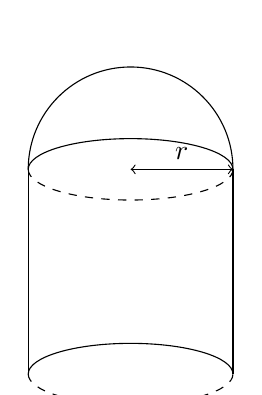
\begin{tikzpicture}[scale=1.3]
            % cylinder side edges
            \draw (-1,0) -- (-1,2);
            \draw (1,0) -- (1,2);

            % bottom ellipse (base of cylinder): back dashed, front solid
            \draw[dashed] (-1,0) arc (180:360:1 and 0.3);
            \draw (-1,0) arc (180:0:1 and 0.3);

            % top ellipse (junction of cylinder & hemisphere): front solid, back dashed
            \draw (-1,2) arc (180:0:1 and 0.3);
            \draw[dashed] (-1,2) arc (180:360:1 and 0.3);

            % hemisphere dome (visible silhouette)
            \draw (-1,2) arc (180:0:1 and 1);

            % radius label
            \draw[<->] (0,2) -- (1,2) node[midway, above]{$r$};
        \end{tikzpicture}
    \end{center}

    \begin{enumerate}[label=(\roman*)]
        \item 若 $\dfrac{dr}{dt}=0.1\text{ cm/s}$，当 $r=4\text{ cm}$ 时，求此立体表面积的变率。 \qscore{3}

        \item 当 $r\to0^+$，$V$ 与 $S$ 各有什么变化？ \qscore{3}
    \end{enumerate}

    \item 用换元积分法或其他方法，求 $\displaystyle\int_0^4 (x-1)(x^2-2x+2)^3\,dx$。 \qscore{4}
    \end{questionparts}
\end{question}

\begin{solution}
    \begingroup\compactanswers
    \begin{enumerate}[label=(\alph*)]
        \item 求表面积的变率 $\dfrac{dS}{dt}$。 \\
        先求 $\dfrac{dS}{dr}$：
        \[
            \frac{dS}{dr}=6\pi r-\frac{288\pi}{r^2}
        \tag*{(1分)}
    \]
        代入 $r=4$：
        \begin{align*}
            \frac{dS}{dr}\bigg|_{r=4} &= 6\pi(4)-\frac{288\pi}{16} \\
            &= 24\pi-18\pi=6\pi
        \tag*{(1分)}
        \end{align*}
        由链式法则：
        \[
            \frac{dS}{dt}=\frac{dS}{dr}\times\frac{dr}{dt}=6\pi\times0.1=0.6\pi\text{ cm}^2/\text{s}
        \tag*{(1分)}
    \]

        \item 分析当 $r\to0^+$ 时 $V$ 与 $S$ 的变化。 \\
        对于 $V=144\pi+\dfrac{2}{3}\pi r^3$：当 $r\to0^+$，$r^3\to0$，故
        \[
            V\to144\pi\ (\text{趋向一个有限值})
        \tag*{(1分)}
    \]
        对于 $S=3\pi r^2+\dfrac{288\pi}{r}$：当 $r\to0^+$，$3\pi r^2\to0$，但 $\dfrac{288\pi}{r}\to+\infty$，故
        \[
            S\to+\infty\ (\text{无限增大})
        \tag*{(1分)}
    \]
        故当 $r\to0^+$ 时，体积 $V$ 趋于有限值 $144\pi$，而表面积 $S$ 则无限增大。
        \qscore[分]{1}
    \end{enumerate}

    \smallskip
    求 $\displaystyle\int_0^4 (x-1)(x^2-2x+2)^3\,dx$。 \\
    设 $u=x^2-2x+2$，则 $du=(2x-2)dx=2(x-1)dx$，故 $(x-1)dx=\dfrac{du}{2}$。
    \qscore[分]{1}\par
    改变积分上下限：当 $x=0$，$u=2$；当 $x=4$，$u=10$。
    \qscore[分]{1}\par
    \[
        \int_0^4 (x-1)(x^2-2x+2)^3\,dx=\int_2^{10} u^3\cdot\frac{du}{2}=\frac12\left[\frac{u^4}{4}\right]_2^{10}
    \tag*{(1分)}
    \]
    \begin{align*}
        &=\frac18\left(10^4-2^4\right)=\frac18(10000-16)=\frac{9984}{8}
    \end{align*}
    \[
        =1248
    \tag*{(1分)}
    \]
    \par\endgroup
\end{solution}
%endregion

\newpage

%region 范围：2026年金宝培元独中高三高级数学(SC05)毕业考·试卷二·乙组 | 考点：乘积求导、换元积分、旋转体体积 | 难度：中等偏难
\begin{question}[points = 10]
    \begin{questionparts}
        \item 已知 $y=x\sqrt{x-1}$，证明 $\dfrac{dy}{dx}=\dfrac{3x-2}{2\sqrt{x-1}}$。据此，求 $\displaystyle\int_4^6 \frac{9x-2}{\sqrt{3x-1}}\,dx$。 \qscore{5}

    \item 下图中的阴影部分是由曲线 $y=8x^3$ 及 $y^2=2x$ 所围成。求此区域绕 $y$ 轴旋转 $360^\circ$ 所形成的旋转体体积。

    \begin{center}
            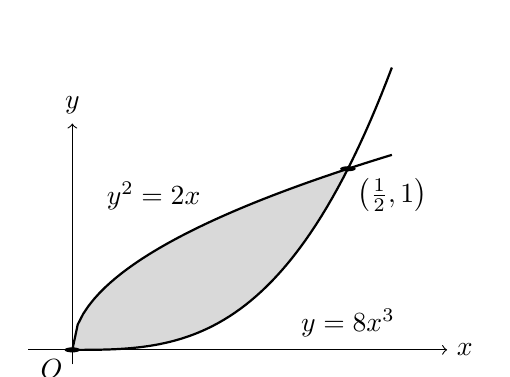
\begin{tikzpicture}[xscale=7, yscale=2.3]
                % 坐标轴
                \draw[->] (-0.08,0) -- (0.68,0) node[right] {$x$};
                \draw[->] (0,-0.08) -- (0,1.25) node[above] {$y$};

                % 阴影区域（两曲线之间，仅到交点为止）
                \fill[gray!30, domain=0:0.5, variable=\x, samples=60]
                    plot ({\x},{sqrt(2*\x)})
                    -- plot[domain=0.5:0, variable=\x] ({\x},{8*\x*\x*\x})
                    -- cycle;

                % 曲线，延伸超过交点
                \draw[domain=0:0.58, samples=60, thick] plot ({\x},{sqrt(2*\x)});
                \draw[domain=0:0.58, samples=60, thick] plot ({\x},{8*\x*\x*\x});

                % 交点
                \fill (0,0) circle (0.4pt);
                \fill (0.5,1) circle (0.4pt);
                \node[below left] at (0,0) {$O$};
                \node[below right] at (0.5,1) {$\left(\frac12,1\right)$};

                % 曲线标签
                \node[above left] at (0.25,0.72) {$y^2=2x$};
                \node[below ] at (0.5,0.28) {$y=8x^3$};
            \end{tikzpicture}
        \end{center}


    \qscore{5}
    \end{questionparts}
\end{question}

\begin{solution}
    \begingroup\compactanswers
    \begin{enumerate}[label=(\alph*)]
        \item 证明 $\dfrac{dy}{dx}=\dfrac{3x-2}{2\sqrt{x-1}}$，并据此求积分。 \\
        利用乘积法则，$y=x\sqrt{x-1}$：
        \begin{align*}
            \frac{dy}{dx} &= (1)\sqrt{x-1}+x\cdot\frac{1}{2\sqrt{x-1}} \\
            &= \sqrt{x-1}+\frac{x}{2\sqrt{x-1}}
        \tag*{(1分)}
        \end{align*}
        通分化简：
        \begin{align*}
            \frac{dy}{dx} &= \frac{2(x-1)+x}{2\sqrt{x-1}}=\frac{3x-2}{2\sqrt{x-1}}\quad\checkmark
        \tag*{(1分)}
        \end{align*}
        据此求积分：设 $t=3x$，则 $dt=3\,dx$，且当 $x=4,6$ 时 $t=12,18$。 \\
        注意 $t-1=3x-1$，$3t-2=9x-2$，恰与被积式吻合：
        \[
            \int_4^6\frac{9x-2}{\sqrt{3x-1}}dx=\int_{12}^{18}\frac{3t-2}{\sqrt{t-1}}\cdot\frac{dt}{3}
            =\frac23\int_{12}^{18}\frac{3t-2}{2\sqrt{t-1}}dt
        \tag*{(1分)}
    \]
        由 (a) 的结果，$\displaystyle\int\frac{3t-2}{2\sqrt{t-1}}dt=t\sqrt{t-1}+C$，故：
        \[
            =\frac23\Big[t\sqrt{t-1}\Big]_{12}^{18}=\frac23\Big[3x\sqrt{3x-1}\Big]_4^6=\Big[2x\sqrt{3x-1}\Big]_4^6
        \tag*{(1分)}
    \]
        \begin{align*}
            &= 2(6)\sqrt{17}-2(4)\sqrt{11} \\
            &= 12\sqrt{17}-8\sqrt{11}
        \tag*{(1分)}
        \end{align*}

        \item 求旋转体体积。 \\
        求两曲线交点：将 $y=8x^3$ 代入 $y^2=2x$：
        \[
            64x^6=2x\ \Rightarrow\ 2x(32x^5-1)=0\ \Rightarrow\ x=0\ \text{或}\ x=\frac12
        \]
        对应 $y=0$ 或 $y=1$，交点为 $(0,0)$ 及 $\left(\dfrac12,1\right)$。
        \qscore[分]{1}\par
        绕 $y$ 轴旋转，须将两曲线表示为 $x$ 关于 $y$ 的函数：
        \[
            y=8x^3\ \Rightarrow\ x=\frac{y^{1/3}}{2};\qquad y^2=2x\ \Rightarrow\ x=\frac{y^2}{2}
        \]
        在 $0<y<1$ 时，$\dfrac{y^{1/3}}{2}>\dfrac{y^2}{2}$，故外半径 $R(y)=\dfrac{y^{1/3}}{2}$，内半径 $r(y)=\dfrac{y^2}{2}$。
        \qscore[分]{1}\par
        利用垫圈法（washer method）：
        \[
            V=\pi\int_0^1\Big[R(y)^2-r(y)^2\Big]dy=\pi\int_0^1\left(\frac{y^{2/3}}{4}-\frac{y^4}{4}\right)dy
        \tag*{(1分)}
    \]
        \begin{align*}
            &=\frac{\pi}{4}\left[\frac{3}{5}y^{5/3}-\frac15 y^5\right]_0^1
            =\frac{\pi}{4}\left(\frac35-\frac15\right)
        \tag*{(1分)}
        \end{align*}
        \[
            V=\frac{\pi}{4}\times\frac25=\frac{\pi}{10}
        \tag*{(1分)}
    \]
    \end{enumerate}
    \par\endgroup
\end{solution}
%endregion

\vfill % 与上方内容保持距离

\noindent
\newlength{\sigwidth}
\settowidth{\sigwidth}{（\hspace{4em}师）}

\begin{tabular*}{\textwidth}{@{\extracolsep{\fill}} l l l}
    出题： & 审题： & 审核： \\[4em]
    \rule{\sigwidth}{0.5pt} &
    \rule{\sigwidth}{0.5pt} &
    \rule{\sigwidth}{0.5pt} \\
    （\hspace{0em} \setterteacher ） &
    （\hspace{0em} \reviewteacher ）  &
    （\hspace{0em} \auditteacher ） \\
\end{tabular*}

\clearpage
\thispagestyle{empty} % 取消这一页的页眉页脚（页码）
~
\clearpage
\end{document}
